\documentclass[12pt]{report}
\usepackage[a4paper]{geometry}
\usepackage[myheadings]{fullpage}
\usepackage{fancyhdr}
\usepackage{graphicx, wrapfig, subcaption, setspace, booktabs}
\newcommand{\HRule}[1]{\rule{\linewidth}{#1}}
\onehalfspacing
\setcounter{tocdepth}{5}
\setcounter{secnumdepth}{5}
\usepackage[english]{babel}
\usepackage{algorithm}
\usepackage[noend]{algpseudocode}
\pagestyle{fancy}
\fancyhf{}
\setlength\headheight{15pt}
\fancyhead[R]{ETERNITY : FUNCTION : log_{b}(x)}



\begin{document}

\title{ \Large \text{{SOEN-6011   SOFTWARE ENGINEERING PROCESS}}
		\\ [2.0cm]
		\HRule{2pt} \\ [0.5cm]
		\LARGE \textbf{\uppercase{ETERNITY : function : log_{b}(x)}}\\
		\HRule{2pt} \\ [0.5cm]
		\textbf{{\Large Deliverable 1}}\\
		\normalsize  \vspace*{5\baselineskip}}

\date{}
\author{\LARGE \textbf{
		SAHANA ANANTHA \\
		\Large \text{Student Id} : \text{ 40085533}\\
        \Large \text{Guided By} - Prof. PANKAJ KAMTHAN  \\
\Large \text {CONCORDIA UNIVERSITY}\\
\small \text  https://github.com/SahanaAnantha/SOEN-6011 \\}}

\maketitle

\newpage
\tableofcontents
\pagebreak
\renewcommand{\thesection}{\arabic{section}}

\section{Introduction}
\subsection{Description}

A logarithmic answer the question " How many of this number do we multiply to get that number? " 

    For Example:  How many 2s must we multiply to get 8?\\
    $$Ans: 2 * 2 * 2$$
    So we had to multiply 3 of the 2s to get 8 \\We say the logarithm of 8 with base 2 is 3 \\
    In fact, these two things are the same:
		2 * 2 * 2  is equivalent to $log_2 (8) = 3$

\subsection{Definition}
A logarithm is an exponent which indicates to what power a base must be raised to produce a given number.
The logarithm of x in the base b is written $log_b (x)$ and is defined as,
$$log_b (x) = y$$
\begin{center}
if and only if $by = x$, where $x > 0$ and $b > 0$, $b\neq1$
\end{center}

\begin{center}
 logarithmic form :  $log_b (x)$
\end{center}

\begin{center}
exponential form : $b^y = x$
\end{center}


\subsection{Domain}
    
    \begin{center}
      Set of positive real numbers  $ x > 0 $
    \end{center}
    
\subsection{Co-Domain}
\begin{center}
    Set of real numbers R from $-\infty$  to $+\infty$\\[0.5 cm] 
\end{center}

\begin{figure}[h!]
\begin{center}
  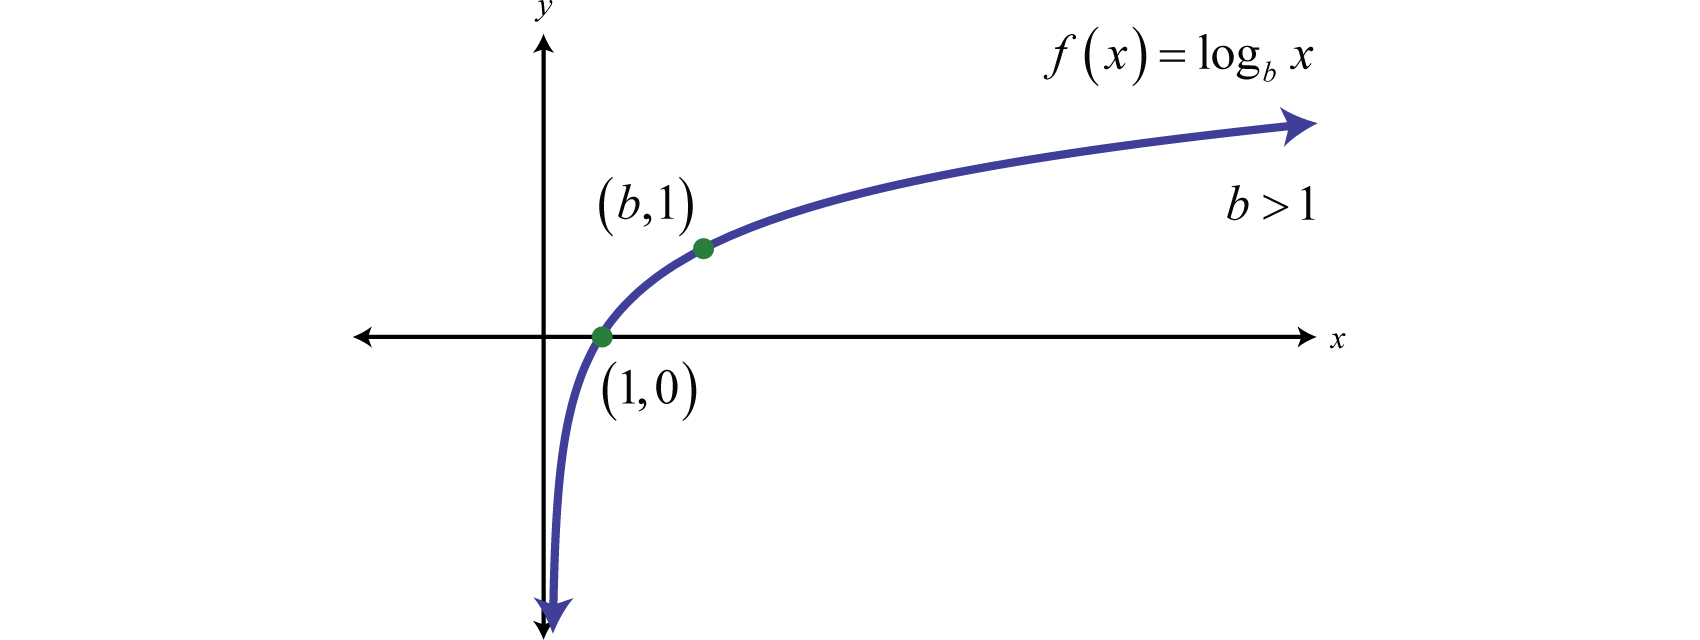
\includegraphics[width=\columnwidth]{Log.png}
  \end{center}
  \caption{Graph of logarithmic function (Source: Google Images)}
\end{figure}


\section{Functional Requirement}
\subsection{Assumption}
\begin{itemize}
\item ID: 1
\begin{itemize}
\item Description: The function $log_b (X)$ has two inputs that is b and X
\end{itemize}
\item ID: 2
\begin{itemize}
\item Description: Output of the function $log_b (X)$ is a Real Number
\end{itemize}
\item ID: 3
\begin{itemize}
\item Description: For out of range values of input , the output is undefined and throws error
\end{itemize}
\end{itemize}

\subsection{Requirements}
\begin{itemize}
\item ID: RQ1
\begin{itemize}
\item Version:  1.0
\item Type: Functional Requirement
\item Priority: 1
\item Risk: High
\item Description: The user has to input the valid X and b values
\item Rationale: The input values provided by the user should be within the domain specified
\end{itemize}
\item ID: RQ2
\begin{itemize}
\item Version:  1.0
\item Type: Functional Requirement
\item Priority: 1
\item Risk: High
\item Description: When either the value of X or b are missing, the system should display error
\item Rationale: X and b are the mandatory input for log function
\end{itemize}
\item ID: RQ3
\begin{itemize}
\item Version:  1.0
\item Type: Functional Requirement
\item Priority: 1
\item Risk: High
\item Description: The value of b should be greater than 1.
\item Rationale: If the value of b is 0 the result would be undefined
\end{itemize}
\item ID: RQ4
\begin{itemize}
\item Version:  1.0
\item Type: Functional Requirement
\item Priority: 2
\item Risk: medium
\item Description: The console will display the result in stipulated time
\item Rationale: To measure the performance and efficiency.
\\\\
\end{itemize}
\item ID: RQ5
\begin{itemize}
\item Version:  1.0
\item Type: Non- Functional Requirement
\item Priority: 3
\item Risk: Low
\item Description: The console should display appropriate error message when invalid input is given.
\item Rationale: To have better user friendly system
\end{itemize}
\end{itemize}





\pagebreak
\section{Algorithm}
\begin{algorithm}
\caption{Approximation algorithm for LOGARITHM (X, b)}
\textbf{Input: X value $(X > 0)$   ; b value $(b>0, b \neq 1)$  $b=e=2.1782$}\\
\textbf{Output: y has values between $-\infty$ to $+ \infty$ }
\begin{algorithmic}[1]
\Procedure{Approximation}{$X,e$}
\If{$x$ is $>$ 1.0}
  \State $term \gets (X-1)/X$
  \State $denominator  \gets (X-1)/X$
  \State $temp \gets term$

\While{$temp > 1E-15$ }
\State $result\gets result+temp$
\State $term\gets term* (1.0/denominator)$
\State $denominator\gets denominator+1$
\EndWhile\label{algorithmendwhile}
\State \textbf{return} $result$
\EndIf
\If{$x$ is greater 0.0}
  \State $result \gets 0.0$
  \State $term  \gets X-1$
  \State $Power of one \gets -1$
  \State $denominator\gets 2$
  \State $temp  \gets term$
\While{$temp > 1E-15 || -temp > 1E-15$ }
    \If{$temp>1E-15$}
    \State $result\gets result-temp$
    \EndIf
\EndWhile
\EndIf
\State Else
\State $result\gets result+temp$
\State $term\gets term* (X-1)$
\State $temp\gets term* power of 1$
\State $denominator\gets denominator+1$
\State \textbf{return} $result+term$
\State \textbf{return} $result$
\EndProcedure
\end{algorithmic}
\end{algorithm}

\begin{algorithm}
\caption{Algorithm for LOGARITHM (X)}
\textbf{Input: X value $(X > 0)$   ; b value $(b>0, b \neq 1)$  $b=e=2.1782$}\\
\textbf{Output: LnofX has values between $-\infty to + \infty$ }
\begin{algorithmic}[1]
\Procedure{Approximation}${X,e}$
\State $X \gets Input $\Comment{input the value of X}
\State $y \gets \frac{(X-1)}{(X+1)}$
\State $ySquared \gets y*y$
\State $increment \gets 1$
\For{\texttt{(i=1/increment i> .00000000001; increment = increment+2 )}}
        \State $repeatingValue \gets i+ySquared$
        \State $newRepeat \gets repeatingValue$
        \State $finalRepeat \gets newRepeat * repeatingValue$
        \State $LnofX = 2 * y * finalRepeat$
      \EndFor

\EndProcedure
\end{algorithmic}
\end{algorithm}

\pagebreak

\subsection{Description}
For calculating the Logarithmic value , the above two algorithms are selected. 
\subsection{Algorithm 1}
The first one chooses the approximation algorithm which  uses the constant variables as input. In this the value of e that is the Euclid's constant is declared and accordingly the pseudo code tells the way in which the calculation of natural logarithm is made. Similarly the base value is calculated as below. 

$$ log_b(x) = \frac{log_e(x)}{log_e(b)}$$

\subsection{Algorithm 2}
The second algorithm for the Logarithmic function has the steps to  calculate the value of log with base e. With the help of these steps the logarithm value to different base values can be calculated.The result calculated will be in decimals. 

$$ log_b(x) = \frac{log_e(x)}{log_e(b)}$$
\\\\

\subsection{Advantages and Disadvantages}
\textbf{Advantages}
\begin{itemize}
   \item Algorithm1 provides the more accurate results for the value of x with in the domain
   \item The values can be separated and calculated for each input using the natural logarithm 
   \item Execution is faster in algorithm1 than algorithm2 which can be estimated from the O notation.
\end{itemize}

\textbf{Disadvantages}
\begin{itemize}
   \item The Algorithm2 uses the for loop with with less precision values which hinders the performance
   
\end{itemize}

\begin{thebibliography}{9}
\bibitem{UCC}
University College Cork,
\\\texttt{http://www.cs.ucc.ie/\~dgb/courses/toc/handout26.pdf}

\bibitem{basecs} 
Basecs,
\\\texttt{https://medium.com/basecs/looking-for-the-logic-behind-logarithms-9e79d7666dda}

\bibitem{wiki} 
Wikipedia,
\\\texttt{https://en.wikipedia.org/wiki/Natural\_logarithm\#Numerical\_value}

\bibitem{University of Sydney}
University of Sydney,
\\\texttt{https://magma.maths.usyd.edu.au/magma/handbook/text/194}
\end{thebibliography}
\end{document}

